\chapter{Aplicación}
\label{cap:descripcionTrabajo}

\section{Back-end}
Una parte muy importante de nuestro trabajo es brindar una aplicación con la cual, cualquier usuario tenga la capacidad de utilizar nuestros modelos entrenados, es decir que pueda generar imágenes personalizadas de cualquier elemento que desee. El objetivo es aportar un valor añadido a nuestro trabajo, para que los destinatarios puedan, no solo obtener la mejor manera de crear imágenes personalizadas, sino que dispongan de una plataforma donde poder obtener todos los resultados deseados.\\

Para la creación de la aplicación optamos por realizar el código de diferentes formas, la primera de ellas siendo todo en lenguaje Python. Con esto se logró un buen resultado a nivel de funcionalidad, pues generaba las imágenes deseadas en el mismo tiempo en el que se generan en la aplicación SDGUI, previamente mencionada. No obstante, no logramos que la aplicación tuviese una interfaz atractiva e intuitiva para el usuario.\\

\begin{figure}[!htb]
	\centering
	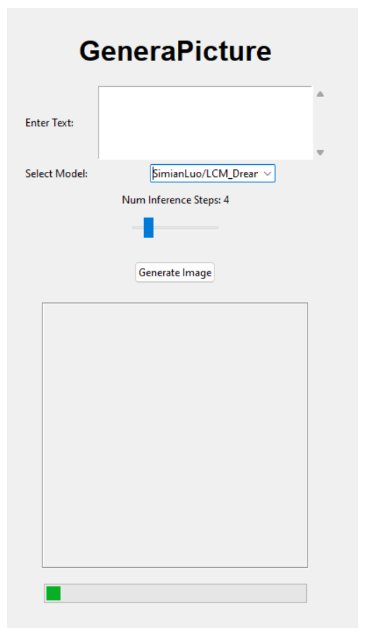
\includegraphics[width = 0.7
	\textwidth]{Imagenes/Vectorial/app1.png}
	\caption{Prototipo de la aplicación en Python}
	\label{fig:app1}
\end{figure}

De este modo, decidimos utilizar una vía mejor para poder centrarnos por un lado en el estilo, y por otro lado en la funcionalidad. Para la lógica o funcionamiento de la generación de imágenes, realizamos un script en Python (app.py), lo que sería el backend del programa. Por otro lado, para el diseño y para solicitar al usuario los datos de entrada, creamos un script en html (index.py). En esta parte del código, se hizo un diseño de la interfaz de la aplicación, es decir, de qué manera queríamos que el usuario genere las imágenes y obtuviese los resultados. Como hemos mencionado con anterioridad, existen una serie de parámetros que son fundamentales para generar una imagen con inteligencia artificial, que son: la descripción (qué queremos que se muestre en la fotografía), el número de pasos o steps (iteraciones en el proceso de creación de la imagen) y el CFG Scale (la medida en la que la ia se debe guiar por la descripción introducida). Estos parámetros, deben ser introducidos por el usuario para la generación. En el método POST del script de Python, obtenemos las indicaciones introducidas por el usuario y se mandan al método Pipeline, que es el encargado de generar el modelo mediante el modelo cargado.\\

Esta aplicación ha tenido dos fases diferenciadas. En la primera, el modelo únicamente funcionaba con un modelo pre entrenado, es decir con un modelo instalado no personalizado, como el Stable Diffusion 1.5. Esto generaba buenos resultados, pero consideramos que no era lo suficientemente útil para poder ser utilizada en el futuro para los libros de vida. Nos encontramos en un punto del proyecto en el que habíamos conseguido entrenar modelos y generar buenas imágenes personalizadas y en el que teníamos un prototipo de aplicación que funcionaba con modelos obtenidos de Hugging Face. Por tanto, el objetivo en esta fase era unir ambas partes que se habían conseguido, y desarrollar un programa con una interfaz atractiva, y con el que se puedan conseguir fotografías adaptadas a cualquier persona. \\

Este fue uno de nuestros mayores retos, puesto que no existía ninguna referencia de cómo utilizar un modelo entrenado para generar una imagen. Era algo particular y que supuso mucho esfuerzo. Para hacer funcionar un modelo de generación de imágenes en un dispositivo local, se necesitan dos librerías: diffusers y torch. La primera, es la que contiene los modelos de Stable Diffusion y derivados o entrenamientos del mismo. La segunda, es la que se encarga de enviar este modelo a la GPU del computador y hacer que se pueda iniciar la generación de la imagen si se encuentra disponible. \\

\begin{figure}[!htb]
	\centering
	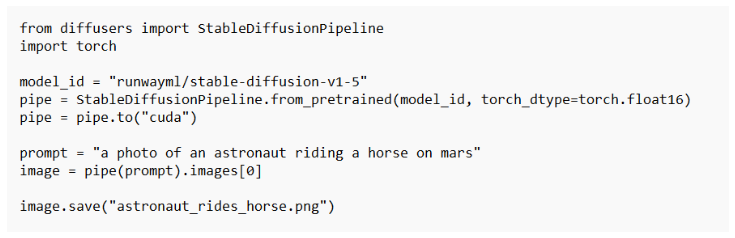
\includegraphics[width = 1
	\textwidth]{Imagenes/Vectorial/codigoapp.png}
	\caption{Funcionamiento de modelos de Stable Diffusion}
	\label{fig:codigoapp}
\end{figure}


Diffusers contiene un método, llamado from pretrained, a través del cual, partiendo de un modelo de los que llamamos pre entrenados, crea una tubería con la lógica del funcionamiento del propio modelo para después ser ejecutado. Nuestro problema  en ese momento, consistía en que este método from pretrained, únicamente aceptaba modelos de la plataforma Hugging Face, pues como parámetro se incluye el PATH de la Web donde se encuentra el modelo. Nosotros persistimos en incluir uno de nuestros modelos propios, pero la carga del archivo en formato .ckpt no era correcta con ninguno de los métodos utilizados, y no se creaba la tubería de manera satisfactoria. \\

No obstante, dimos con una idea que permitía utilizar cualquier modelo entrenado por nosotros mismos. Después de una exhaustiva búsqueda de diferentes bibliotecas de diffusers, encontramos una llamada StableDiffusionPipeline que permite realizar el proceso de crear la tubería, similar al que realiza el método from pretrained, pero en lugar de partir de un modelo pre entrenado, lo hace del enlace a un archivo concreto, que puede ser en formato .ckpt. Este método se llama from single file y como indica su propio nombre en inglés, tan solo necesita un único archivo para hacer funcionar el modelo.\\

Sin embargo, para poder utilizar nuestro propio modelo, se necesitaba un enlace web, no una ruta de archivo. Por tanto, lo que decidimos finalmente fue subir nuestros archivos entrenados en formato .ckpt a Hugging Face, creando una nube personal que incluye todos los entrenamientos realizados. El proceso de subir el archivo es rápido, dependiendo de la conexión a internet, pero si esta es aceptable, en menos de un minuto ya se ha completado con éxito. Al probar la aplicación, la primera vez que se utiliza un modelo entrenado, se debe instalar este en el entorno en el que se está ejecutando. A partir de esto, se generan imágenes con completa normalidad, y de esta manera hemos logrado generar imágenes personalizadas en una aplicación propia.\\

\begin{figure}[!htb]
	\centering
	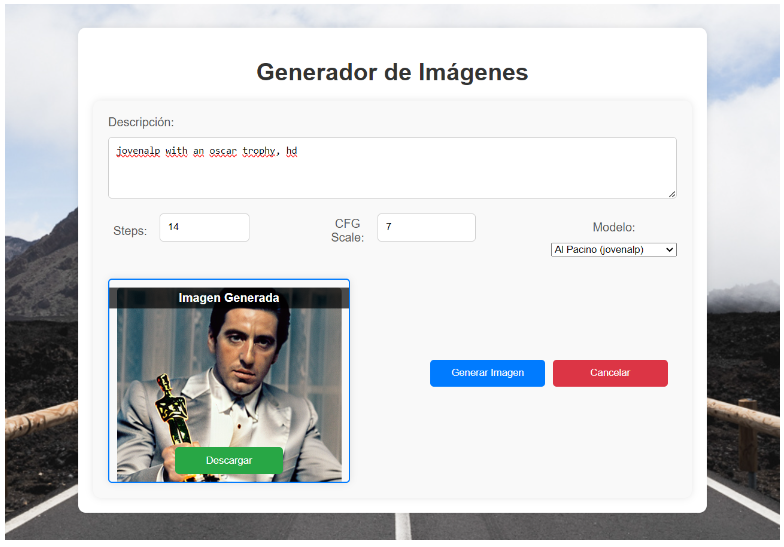
\includegraphics[width = 1
	\textwidth]{Imagenes/Vectorial/genapp.png}
	\caption{Aplicación generadora de imágenes}
	\label{fig:appgen}
\end{figure}




\section{Ejecución de la aplicación}

La manera de utilizar esta aplicación generadora de imágenes es muy sencilla, pero requiere de una explicación para que el usuario pueda hacer uso de ella. En primer lugar, cabe destacar que existe una serie de requisitos para poder utilizar este programa. El primero y más importante, es que, al igual que con la utilización de cualquier modelo de Stable Diffusion en local, se requiere una tarjeta gráfica con un mínimo de 3 gigabytes de memoria virtual. Este es un requisito indispensable, sin el cual se podría acceder a la aplicación pero, en ningún caso, se podría generar ninguna fotografía. Para los usuarios que cuenten con la memoria virtual indicada, se debe contar con una serie de requisitos mínimos, que incluyen las versiones de determinados programas y herramientas necesarias para el funcionamiento de la aplicación.\\

Para saber cuáles eran estos requisitos, creamos un entorno virtual en el que incluimos todo lo relativo a la aplicación. Dentro de este entorno, se creó un archivo llamado dependencies.txt, con el objetivo de que los usuarios descarguen todo lo imprescindible ejecutando el siguiente comando en memoria: pip install -r dependencies.txt. Una vez instalado todo lo necesario, los usuarios deben seguir el proceso que se muestra en la siguiente imagen. En la consola, se debe acceder en primer lugar a la carpeta de nuestro trabajo, llamada tfg, y después al entorno virtual mencionado. Para arrancar el servidor, se debe ejecutar el comando “python app.py”, que como hemos explicado, es el script que recibe los parámetros introducidos por el usuario y los envía a la GPU para generar la imagen y posteriormente mostrarla. Cuando se ha iniciado el servidor, se notifica que está funcionando en el puerto localhost, al cual se puede acceder mediante el navegador, indicando “http://127.0.0.1:5000/”, según aparece indicado. \\
\begin{figure}[!htb]
	\centering
	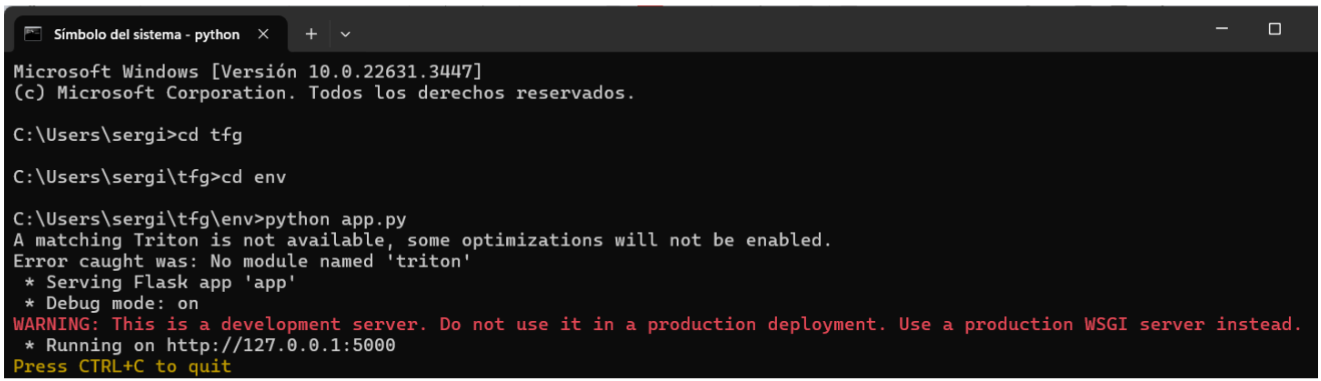
\includegraphics[width = 1
	\textwidth]{Imagenes/Vectorial/exeapp.png}
	\caption{Ejecución de la app}
	\label{fig:appexe}
\end{figure}

A continuación como se muestra en la figura \ref{fig:portadapp} se abrirá nuestra aplicación, donde se ven reflejados dos botones. El primero, para acceder a un libro de vida, donde un hipotético usuario registrado, podrá consultar un libro formado por imágenes generadas por nuestra aplicación, que relatan de manera gráfica momentos únicos, personales y emocionales de la vida del paciente. Es una manera de mostrar los resultados de nuestro proyecto, y lo que cualquier usuario podría conseguir si utiliza nuestra aplicación. \\

El segundo botón accede a nuestra plataforma generadora de imágenes, es decir, lo que se muestra en la imagen anterior. En este caso, el usuario ya está listo para generar su imagen personalizada. Solo debe introducir la descripción, los pasos y la escala CFG, además del modelo entrenado, que incluirá el o los elementos correspondientes de los que se quiere generar la fotografía. Si es la primera vez que se utiliza un determinado modelo, al pulsar en generar imagen se descarga en el entorno, lo cual supone un tiempo de menos de 1 minuto con una conexión a internet aceptable. A continuación, se genera la imagen con una duración dependiente del número de pasos introducidos y de la tarjeta gráfica de cada usuario. En este caso, en nuestro equipo, la generación tiene una duración de entre 10 y 16 segundos por paso introducido, lo que supone un tiempo de unos 3 minutos en una imagen de 15 pasos, que nos aporta una calidad aceptable. Una vez generada la imagen aparecerá reflejada en la aplicación, y el usuario tendrá la posibilidad de descargarla con el nombre que desee.\\

\begin{figure}[!htb]
	\centering
	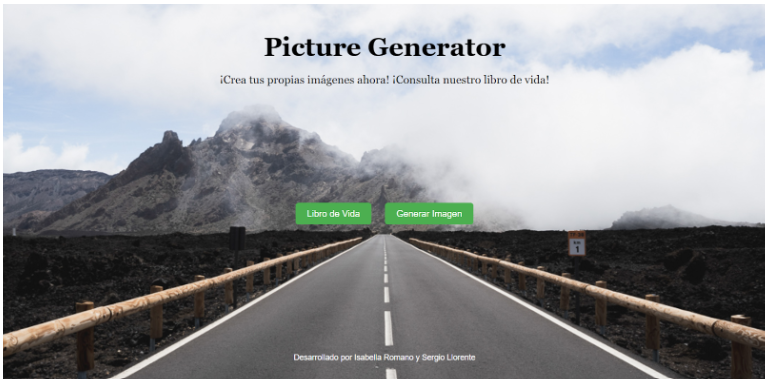
\includegraphics[width = 1
	\textwidth]{Imagenes/Vectorial/portadapp.png}
	\caption{Portada de la aplicación}
	\label{fig:portadapp}
\end{figure}
